\section{Função Objetivo}
A função objetivo $f_U$ é definida pela seguinte
expressão:

\begin{dmath}
  f_U = \sum c_i 
\end{dmath}

Onde $\lbrace c_i \rbrace$ é o conjunto formado
por custos e penalizações. São eles:
\begin{enumerate}
  \item Custo do gap
  \item Correção do Gap devido a movimentação da bola
  \item Distância Total dos Moves
  \item Distância Máxima dos Moves 
  \item Mudança do Planejamento da Move Table
  \item Custo do Ataque
  \item Custo dos gap vistos pelos robôs do time
  \item Custo dos gaps vistos pelos robôs adversários
  \item Custo da Defesa
  \item Número de Receptores
  \item Penalização por próximidade do gol do adversário
  \item Penalização por proximidade
\end{enumerate}

Além dos parâmetros listados acima, outros parâmetros
afetam o comportamento do time:
\begin{enumerate}
  \item Gap mínimo para chute à gol
  \item Número de ramificações
\end{enumerate}

Esses parâmetros serão detalhados a seguir.

\subsection{Custo do gap}\label{subsec:custo_gap}
O objetivos deste parâmetro é valorizar \textit{gaps} maiores
de acordo com a soma total dos \textit{gaps} e com o maior \textit{gap}.
O cálculo do \textit{gap} é feito da seguinte maneira:

\begin{dmath} 
 gap{\_}cost = ratio_{TOTAL{\_}MAX{\_}GAP} . \sum gap_i
 + (1 - ratio_{TOTAL{\_}MAX{\_}GAP}) . max{gap_i} 
\end{dmath} 

Os gaps são calculados de acordo com a posição de um determinado robô
e a posição atual da bola. Isso gera um conjunto de segmentos de reta
$\lbrace gap_i \rbrace$.

Este custo afeta diretamente os seguintes custos:
\begin{itemize}
  \item Custo do Ataque
  \item Custo dos gap vistos pelos robôs do time
  \item Custo dos gaps vistos pelos robôs adversários
  \item Custo da Defesa
\end{itemize}

\subsection{Correção do Gap devido a movimentação da bola} 
O objetivo deste parâmetro é incorporar a movimentação
da bola pelo atacante no cálculo do \textit{gap} do gol. Isso é importante,
pois defensores mais
próximos são mais facilmente driblados que defensores mais distantes. Isso
pode ser visualizado na figura \ref{fig:kick_pos_1}, onde foi considerada
uma variação de 15cm. Já na figura \ref{fig:kick_pos_2} foi considerada uma
variação de 0cm na posição da bola. Essa variação é medida na linha normal
à reta formada pela bola e pelo robô em questão.

% TODO: Adicionar gráfico detalhado as contas
%       vide arquivo board.cpp para detalhes de implementação

\begin{figure}[h]
  \centering
  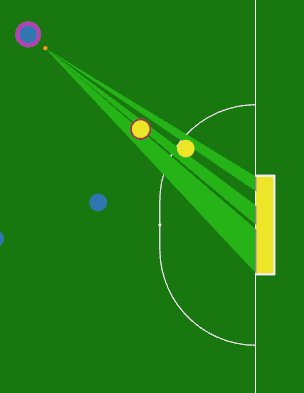
\includegraphics[width=0.5\linewidth]{kick_pos_var_1}
  \caption{\textit{Gap} do gol considerando-se uma variação de 15cm na 
           posição da bola}\label{fig:kick_pos_1}
  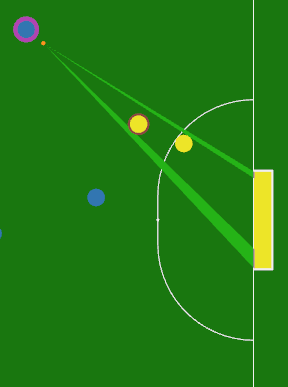
\includegraphics[width=0.5\linewidth]{kick_pos_var_2}
  \caption{\textit{Gap} do gol sem variação de na posição da
           bola}\label{fig:kick_pos_2}
\end{figure}


\subsection{Distância Total dos Moves} 
O objetivo deste parâmetro é valorizar o custo da
mudança de estado na função objetivo. Ele é formado pela soma dos
\textit{moves} de todos os robôs do time em questão.

\begin{dmath} 
 total{\_}move{\_}dist{\_}cost = weight_{MOVE{\_}DIST{\_}TOTAL} . 
 \sum \lVert pos_{r_i} - move_{r_i}\rVert
\end{dmath} 

Onde $r_i \in T$.

\subsection{Distância Máxima dos Moves} 
O objetivo deste parâmetro é incorporar o custo da
mudança de estado na função objetivo. Ele é formado pelo \textit{move}
maior do planejamento atual.

\begin{dmath} 
 max move dist cost = weight_{MOVE{\_}DIST{\_}MAX} . 
 max \lbrace r_i \in T : \lVert pos_{r_i} - move_{r_i}\rVert \rbrace
\end{dmath} 

\subsection{Mudança do Planejamento da Move Table}\label{subsec:change_cost}
O objetivo deste parâmetro é evitar mudanças grandes no
planejamento do move. Uma das razões para isso é evitar um mode dinâmico
exato neste nível de planejamento, já que isso aumentaria muito o custo
computacional desta etapa do planejamento e, consequentemente, reduziria
o número de simulações possíveis. Por essas razões mudanças no planejamento
dos \textit{moves} são penalizadas de acordo com a distância euclidiana
entre o $move_p$ planejado anteriormente e o $move_mr$ modificado.
Isso permite que sejam selecionados $moves_m$ mais próximos do
$move_p$, refinado assim o planejamento anterior.

\begin{dmath} 
 move{\_}change{\_}cost = weight_{MOVE{\_}CHANGE} . 
 max \lbrace \sum_{r_i \in T} \lVert move_{r_i} - move table_{r_i}\rVert \rbrace
\end{dmath} 

\subsection{Custo do Ataque}
Este custo valoriza cituações nas quais o time em questão
possue o domínio da bola (descrito na
subsecção~\ref{subsec:repres_jogo}).

\begin{dmath} 
 attack{\_}cost = weight_{ATTACK} . enemy{\_}gap
\end{dmath} 

Onde $enemy{\_}gap_{value}$ é o valor do gap do goal adversário visto
pelo robô que tem domínio da bola.

\subsection{Custo dos gaps vistos pelos robôs do time}

Este custo tem o objetivo de valorizar configurações nas quais
os robôs que não tem a bola possuam visada para o gol do time
adversário. Isso
é desejavel, já que permite que um gol seja feito caso o robô
que esta com a posse de bola execute um passe para um robô
em questão.

\begin{dmath}
   goal gap of attacker cost = weight_{SEE{\_}ENEMY{\_}GOAL}
    \sum_{r_i \in T_player} enemy{\_}gap_{robot}
\end{dmath}

\subsection{Custo dos gaps vistos pelos robôs adversários}

Este custo é o análogo do custo anterior, mas para o
time adversário. Ele visa penalizar situações nas quais
os robôs adversários tenham grande visada (i.e., gap)
para o gol. 

\begin{dmath}
   goal gap of attacker cost = - weight_{BLOCK{\_}GOAL}
    \sum_{r_i \in T_enemy} player{\_}gap_{robot}
\end{dmath}

\subsection{Custo da Defesa}
Quando não se tem o domínio da bola o gap do time em questão
visto pelo robô do time adversário que tem a bola é utilizado
como penalização adicional.

\begin{dmath}
  defence penalty cost = weight_{BLOCK{\_}ATTACKER}
   \sum_{r_i \in T} player{\_}gap_{robot}
\end{dmath}

\subsection{Número de Receptores}

Este custo visa valorizar cituaçõe nas quais existam
vários robôs que possam receber passe.

\begin{dmath}
  number of recevers cost = weight{\_}RECEIVERS{\_}NUM . 
   num \lbrace recever_i \rbrace
\end{dmath}

\subsection{Penalização por próximidade do gol do adversário}
Esta penalização visa evitar que os robôs que estão no ataque
se concentrem dentro da área do time adversário. Caso este
parâmetro não seja adicionado, é esse o comportamento resultante
do custo dos gap vistos pelos robôs do time em questão. 
A partir de uma determinada distância, é adicionada uma parcela
de penalização na função objetivo.

\begin{dmath}
  custo penalização = - w_{penalização de proximidade} \sum numero de robos perto
\end{dmath}

\subsection{Gap mínimo para chute à gol}
Este parâmetro é o ângulo total do gap do goal para permitir
o chute pelo atacante. Ele é relevante, pois afeta o comportamento
do atacante e, como consequência, o comportamento do time durante
a posse de bola. Quando o gap do gol é menor que este valor, o
atacante tem ação de chutar em direção ao goal.

% TODO: Adicionar imagem para ilustrar este caso, já que não tem
%       equações envolvidas

\subsection{Número da Ramificação}
Este parâmetro é o número de possibilidades que serão simulados
em cada iteração do algorítmo de avaliação. Ele influencia o
tempo de resposta do planejamento.
